\documentclass{article} % For LaTeX2e
% We will use NIPS submission format
\usepackage{nips13submit_e,times}
% for hyperlinks
\usepackage{hyperref}
\usepackage{placeins}
\usepackage{url}
% For figures
\usepackage{graphicx} 
% math packages
\usepackage{amsmath}
\usepackage{amsfonts}
\usepackage{amsopn}
\usepackage{ifthen}
\usepackage{natbib}
\usepackage{caption}
\usepackage{subcaption}

\usepackage{booktabs}
\newcommand{\ra}[1]{\renewcommand{\arraystretch}{#1}}

\title{Convolutional Neural Networks using separable filters}
\author{
\fontsize{8}{8}\selectfont{Petrescu Viviana}\\
\fontsize{8}{8}\selectfont{EPFL} \\
\fontsize{8}{8}\selectfont{\texttt{viviana.petrescu@epfl.ch}} \\
}

\nipsfinalcopy 

\begin{document}

\maketitle

\begin{abstract}
CNN are the state-of-the-art machine learning techniques which achieved best results on various computer vision tasks ranging from the large scale ImageNet object recognition challenge to segmentation in bio medical imaging.
This technical report presents initial results on using CNN with separable filters for speeding up the testing time.
\end{abstract}

\section{Introduction}
Although proven to be very powerful, CNN are much slower for both training and testing than their counter parts SVM or Random Forests.
In the forward pass, the computational complexity of evaluating one image of size $W\times H$ with $J$ filters of size $d_{1}\times d_{2}$ is $O(WHJd_{1}d_{2})$.
 
 Although improving the training time would be very beneficial since it would allow for more configurations to be tried and for larger networks, increasing effort has been put also into speeding up only testing time, since training can be done offline.

\section{Speeding up CNN}
By far the most common approach for speeding up CNNs is to run them on the GPU, making use of the paralelism nature of the algorithm. Alternatively or combined, FFT can be used for the convolutional operations (for  both training and testing)\cite{DBLP:journals/corr/MathieuHL13}.  For testing, a significant speedup can be obtained in hardware by using FGPAs \citep{lecun2010convolutional}. The major drawback of FGPAs is that they are harder to program for people who do not work in the field.

 In \citep{Jaderberg14b} they prove speedup for CNNs for two different schemes using separable filters, one of which is similar with our approach but using a different optimization algorithm for obtaining the separable filters. 
  If the 2d filters are decomposed into a set of separable 1d filters of rank $K$, the complexity per image becomes
 $O(WH(J +d_{1}+d_{2}))$. Thus, we obtain a speedup if $K<< \frac{Jd_{1}d_{2}}{J +d_{1}+d_{2}}$. 
 
 Among the most popular available tools
 - Caffee (C++/GPU) increasingly popular and highly maintained by Berkley Vision group. Higher learning curve but the fastest available tool
 - Theano (Python NumPy C) symbolic differentiation, harder to debug.
 	Easy for small hacks
 - Torch7 (Lua and C) 

\section{Separable filters}
In our approach, the set of filters $\chi$ for one convolutional layer is approximated as
a set of separable filters, as shown in Fig\ref{fig:decomposition}.
\begin{figure}[h]
  \centering
   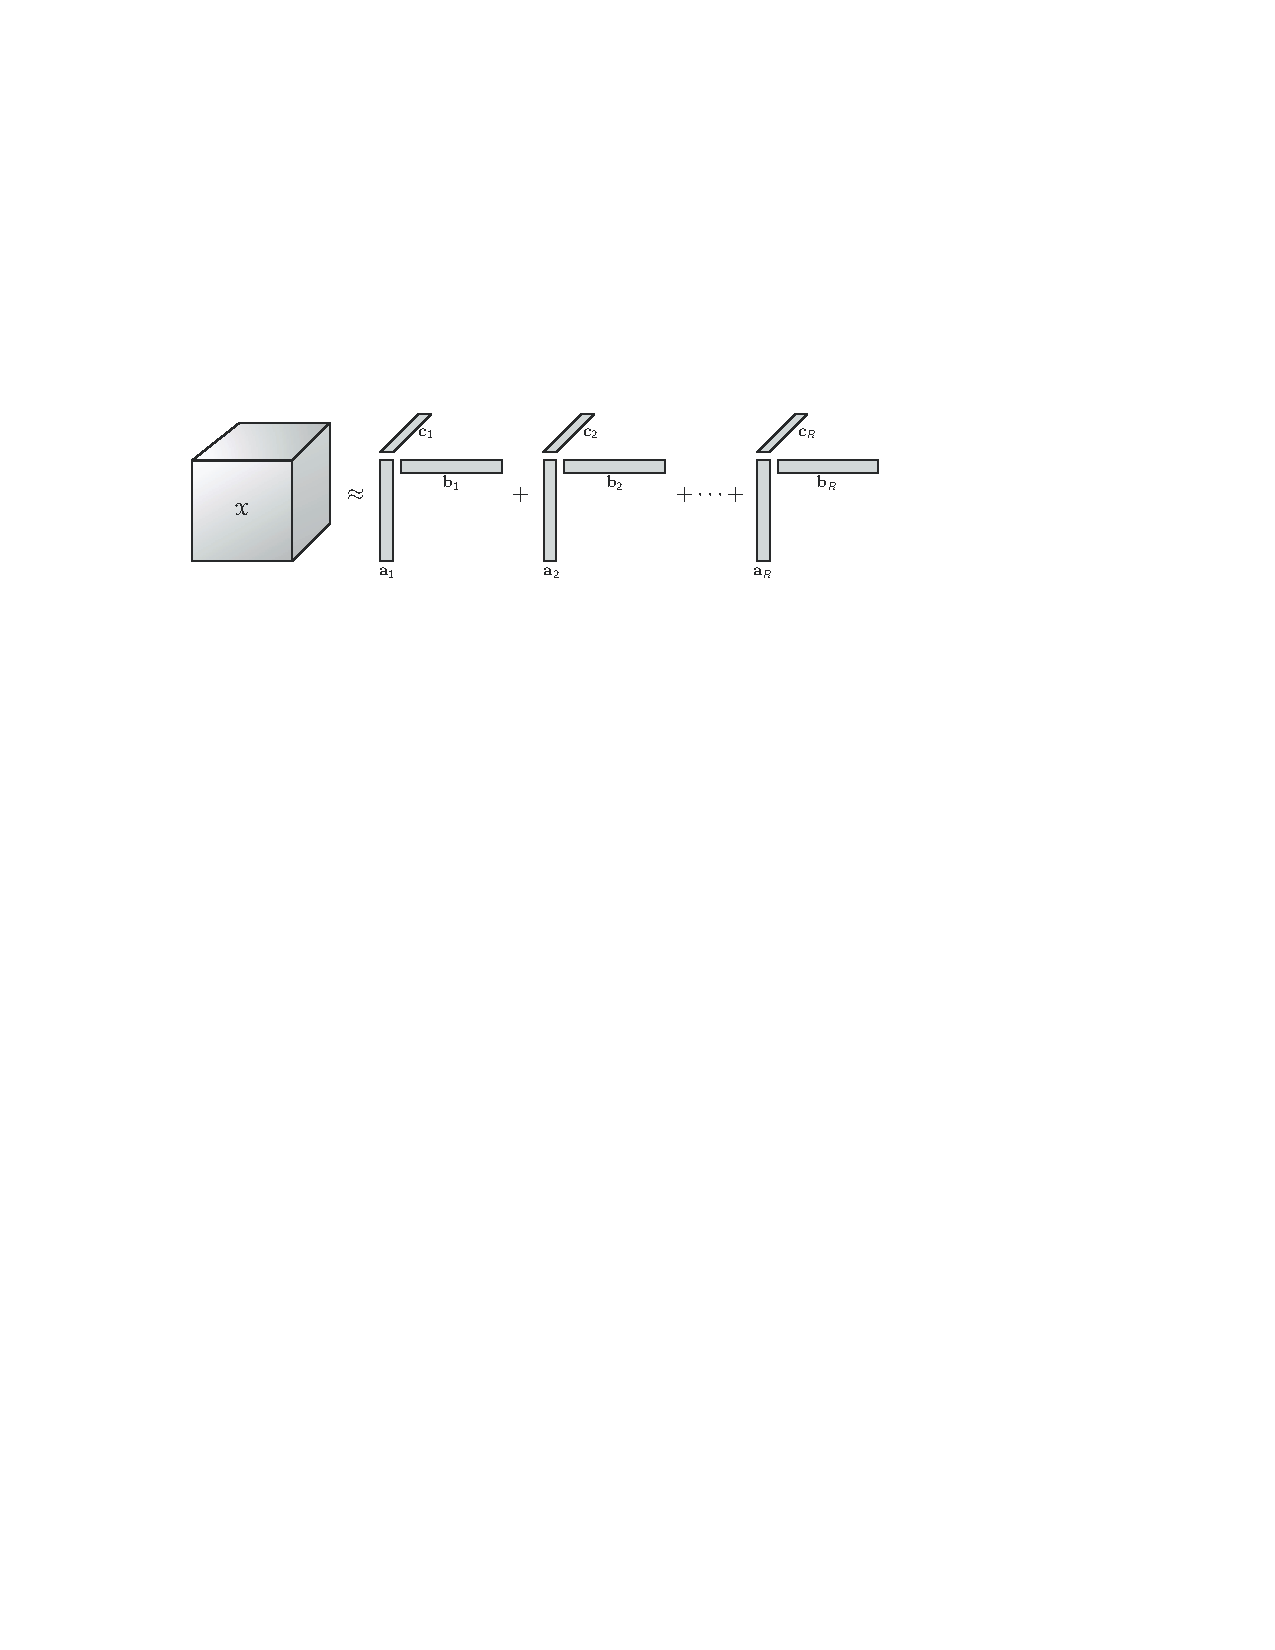
\includegraphics[width=\textwidth]{images/decomposable.pdf}
  \caption{Tensor decomposition}
  \label{fig:decomposition}
\end{figure}

We can obtain an approximation by minimizing the equation:
\begin{equation*}
\begin{aligned}
& \underset{a,b,c}{\text{minimize}}
& \| \chi - \sum_{r=1}^{r=R}{a_{r}\circ b_{r}\circ c_{r}} \|_{2}^{2} 
\end{aligned}
\end{equation*}
We do this using a Matlab implementation of the the Canonical Polyadic decomposition (a generalization of  SVD for tensors),  algorithm which uses non linear conjugate gradient method. The optimization framework requires as input the rank $R$, which is almost never known. When the rank used for decomposition is not the theoretical one, the decomposition is not very accurate and the algorithm needs to be run with different initialization parameter until it converges.
What is known is an upper bound on the theoretical rank $R$ for a  general tensor 3d tensor, given by:
 \begin{equation*}
\begin{aligned}
& \text{rank}(\chi) \leq 
& min{\{IJ, JK, KI\}}
\end{aligned}
\end{equation*} 
Besides the theoretical rank, there is also the notion of typical rank, which is any rank
that appears with probability greater than 0, or that it is most common [cite].
Some of the known typical ranks are shown in Table \ref{table:rank}.
Looking at the first row of Table \ref{table:rank}, we conclude that for a 'very tall' set of filters like the ones present in large CNNs, 
we should expect the rank to be equal with the product of the two kernel dimensions.
 \begin{table}
\centering
\begin{tabular}{@{}ll@{}}\toprule
Tensor size & Typical rank \\ \midrule
$I \times J \times K$ with $JK \leq I$ (very tall) & $JK$\\
$I \times J \times K$ with $JK - J < I < JK$ (tall) & $I$ \\
$I \times J \times K$ with $I = JK - J$ (compact) & $I, I+1$  \\ \bottomrule
\end{tabular}
\caption{Typical rank for certain tensor shapes}
\label{table:rank}
\end{table}

\section{Experiments}
We run the experiments using Theano library in Python. 
We varied the rank for every convolutional layer and compared the separable version with the non separable one. We recorded the time, the change in performance and how well the separable filters approximate the 2d filters. We did this for the MNIST and for the
Mitocondria Striatum datasets.

\subsection{MNIST}
MNIST consists of a curated set of black and white images (28x28) depicting handwritten digits.
The dataset is split into training 60.000 samples, validation 10.000 and testing
10.000 samples. For this set, the approach of \cite{DBLP:journals/corr/abs-1202-2745} using CNNs is the best winning model with a 0.23 error rate (equivalent with 23 out of 10.000 digits not recognized correctly).
We start our experience with the reference Theano model for MNIST which achieves 0.82 error rate. Its configuration is shown in Fig\ref{fig:cnn1}
\subsubsection{Model 1}
\begin{table}
\centering
\begin{tabular}{@{}rlll@{}}\toprule
Layer & Type & Maps and neurons& Kernel size \\ \midrule
0 & input & 1 map of 28x28 &\\
1& convolutional & 20 maps of 24x24 & 5x5\\
2 & max pooling & 20 maps of 12x12 &  \\
3 & convolutional & 50 maps of 8x8& 5x5 \\
4 & max pooling & 50 maps of 4x4&  \\ 
5 & fully conntected& 500 & \\
6 & fully conntected & 2 neurons & \\ \bottomrule
\end{tabular}
\caption{Small CNN for MNIST set}
\label{fig:cnn1}
\end{table}

We first decompose the first convolutional layer1.  From the theoretical point of view, according to Table \ref{table:rank}, we have a compact tensor $R^{20\times 5 \times 5}$ with a typical rank of 20 or 21, so we expect a very good aproximation for rank in that range. 
Fig[ref] shows how well is the approximation with varying rank from 4 to 16 in steps of 2 on the x axis and the fit on the y axis (100 corresponding to perfect fit). As expected, the fit is almost perfect for high ranks and decreases afterwards.

Using separable filters, we obtain a theoretical speedup for conv layer 1 if $K<< \frac{Jd_{1}d_{2}}{J +d_{1}+d_{2}} = 16.66$. Fig\ref{fig:cnn1time}a shows the time improvements using separable filters for conv layer 1. The blue line represents the time per layer using non separable filters. In our implementation, the separable filters give a speedup for any rank, as the red curve is below the blue one. 
We note that that theoretically the non separable time (blue line) and the separable conv with rank 16 should have given the same running time. The reason for the difference is due to implementation details and language specific.

\begin{figure}[h]
  \centering
  \begin{subfigure}[b]{0.40\textwidth}
   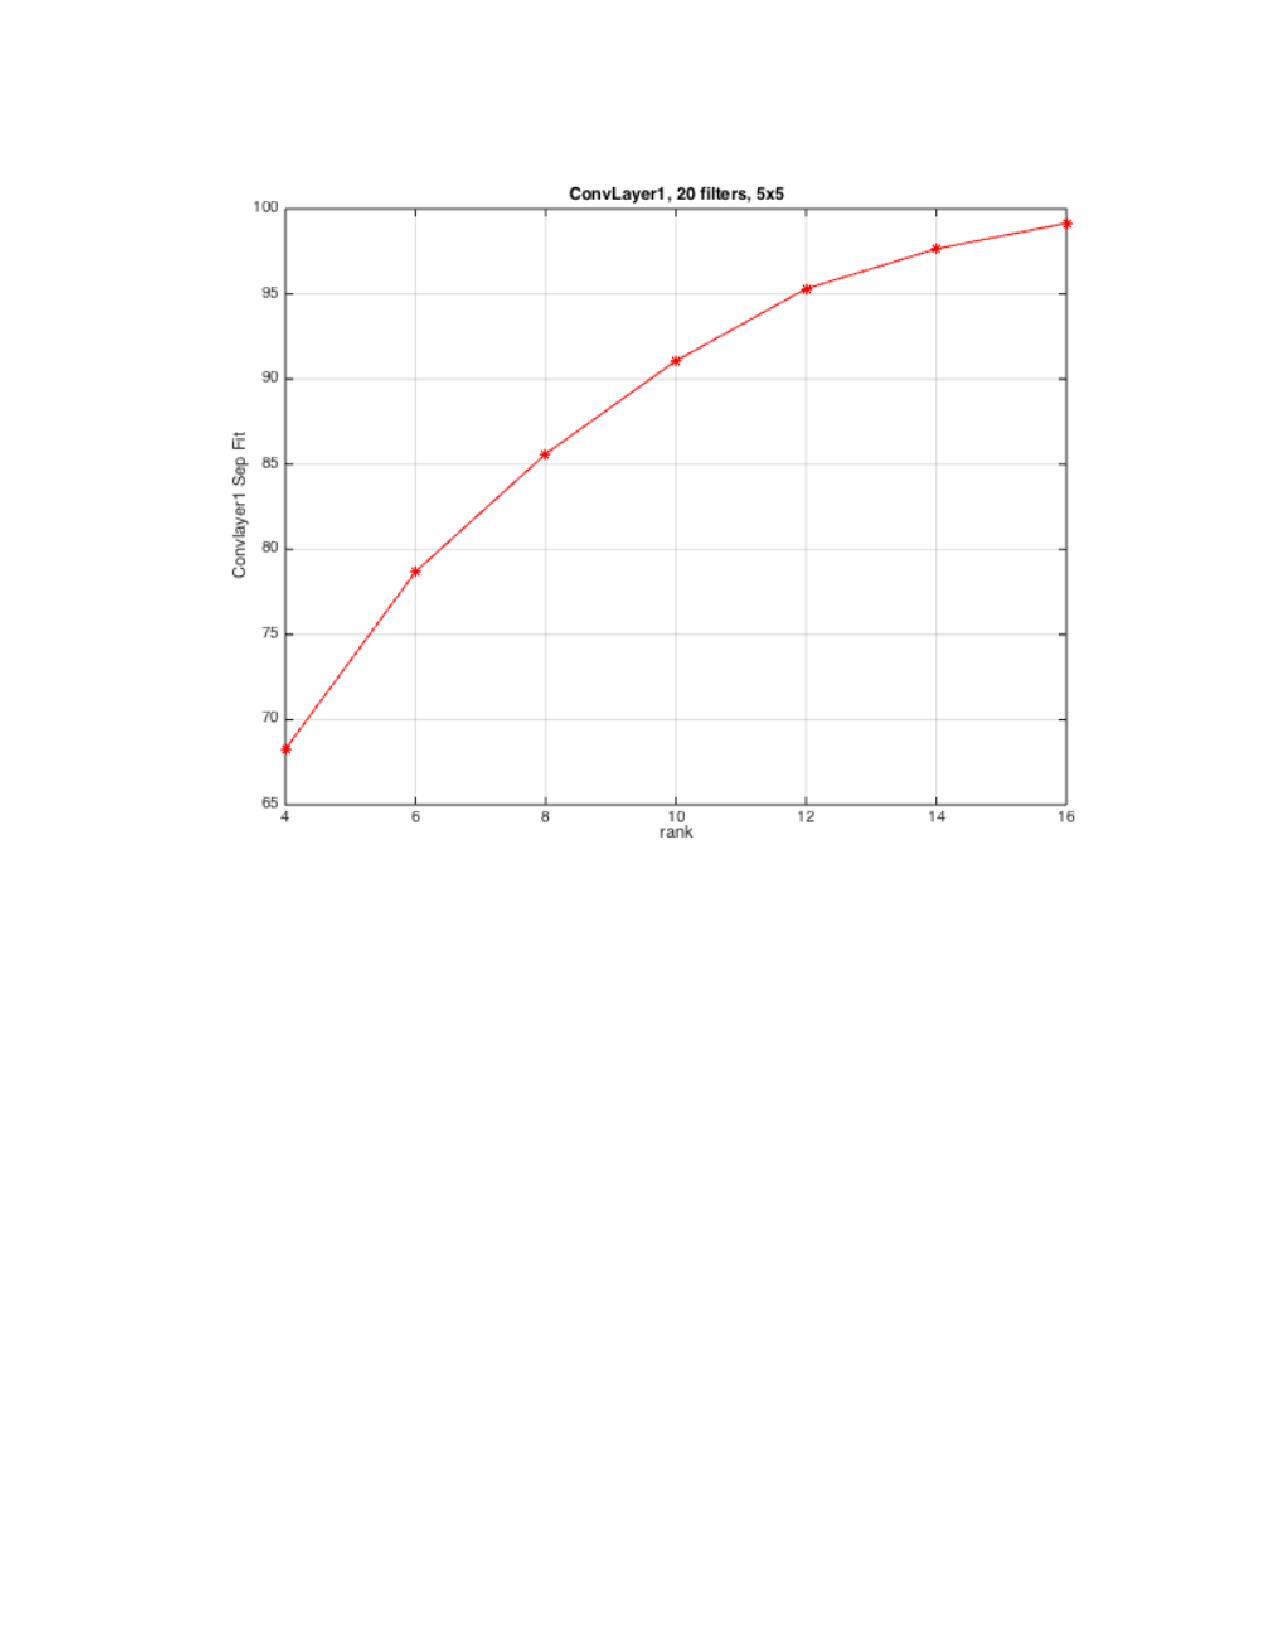
\includegraphics[width=\textwidth]{images/imagesCNN_page6.pdf}
    \caption{Convolutional layer 1}
  \end{subfigure}
  \begin{subfigure}[b]{0.40\textwidth}
    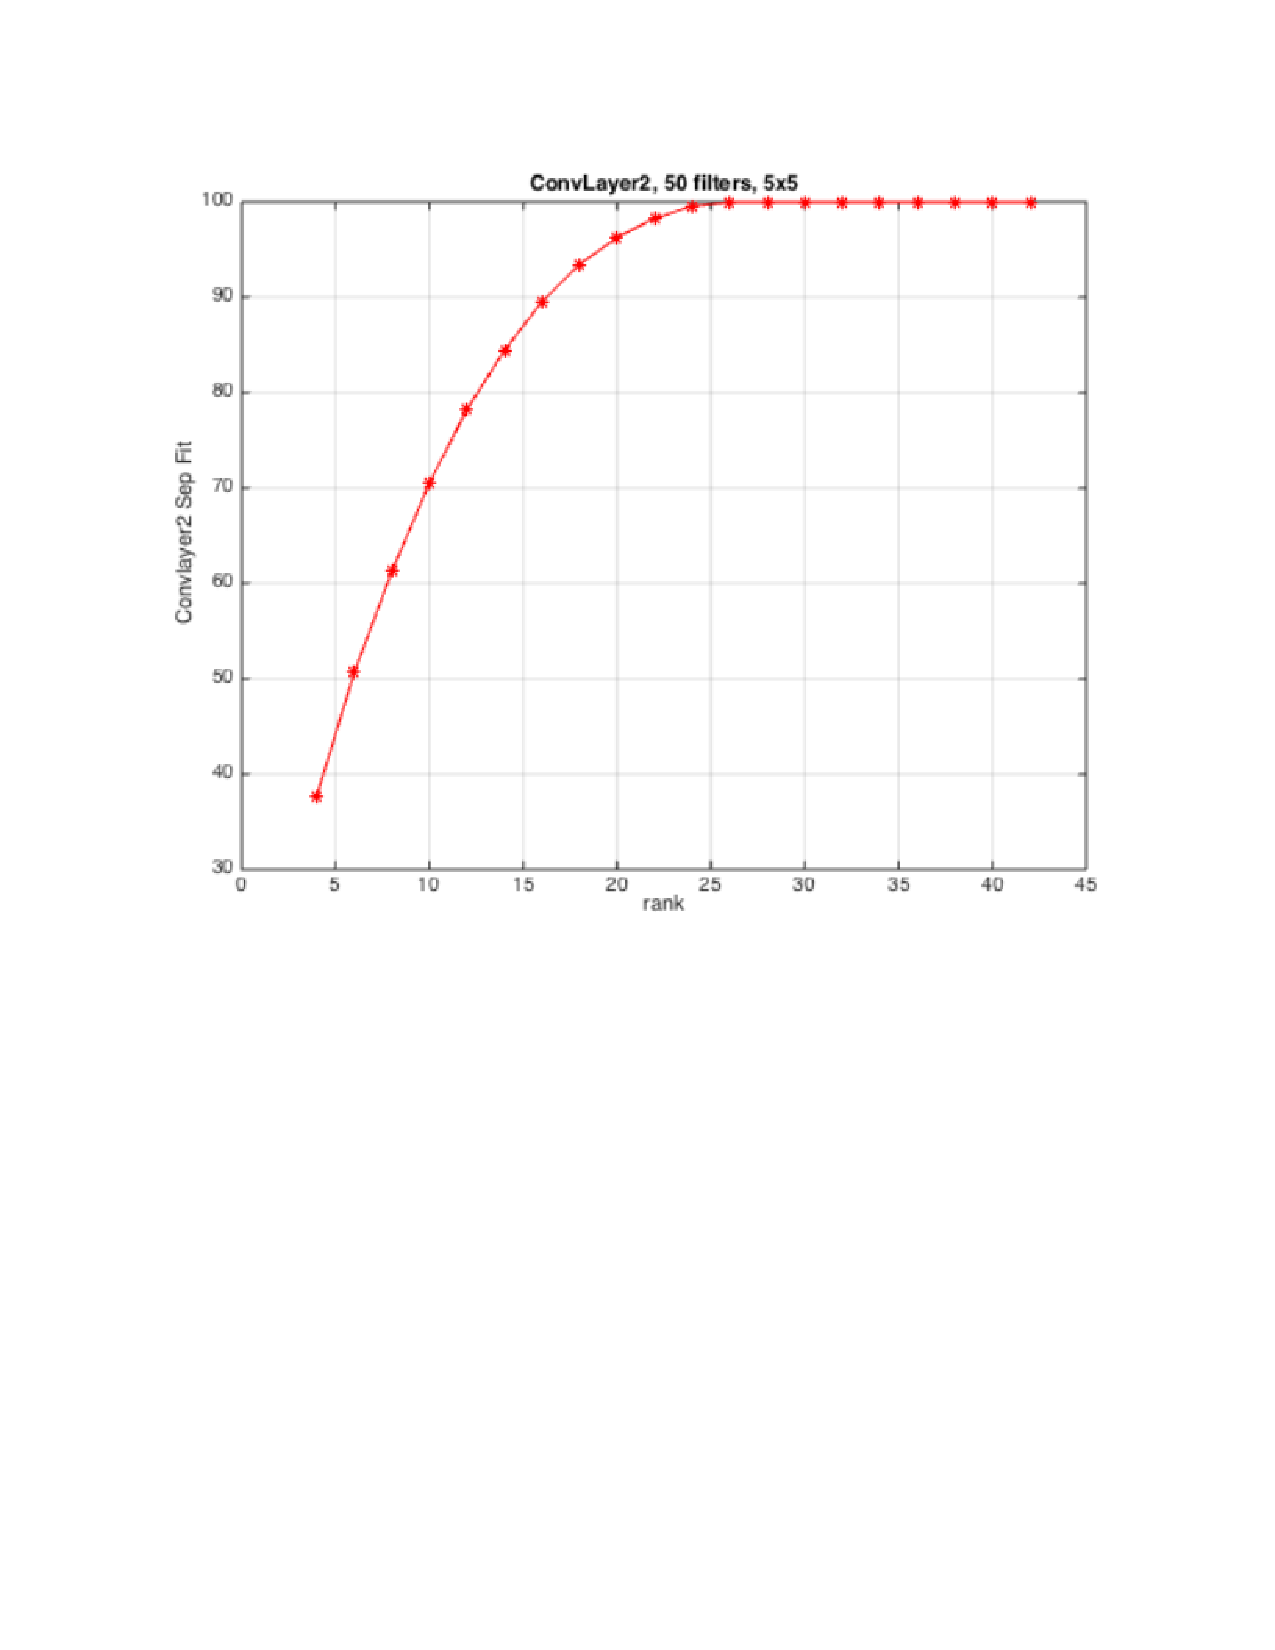
\includegraphics[width=\textwidth]{images/imagesCNN_page2.pdf}
    \caption{Convolutional layer 2}
  \end{subfigure}
  \caption{Rank versus Fit}
  \label{fig:cnn1fitness}
\end{figure}

\begin{figure}[h]
  \centering
  \begin{subfigure}[b]{0.40\textwidth}
   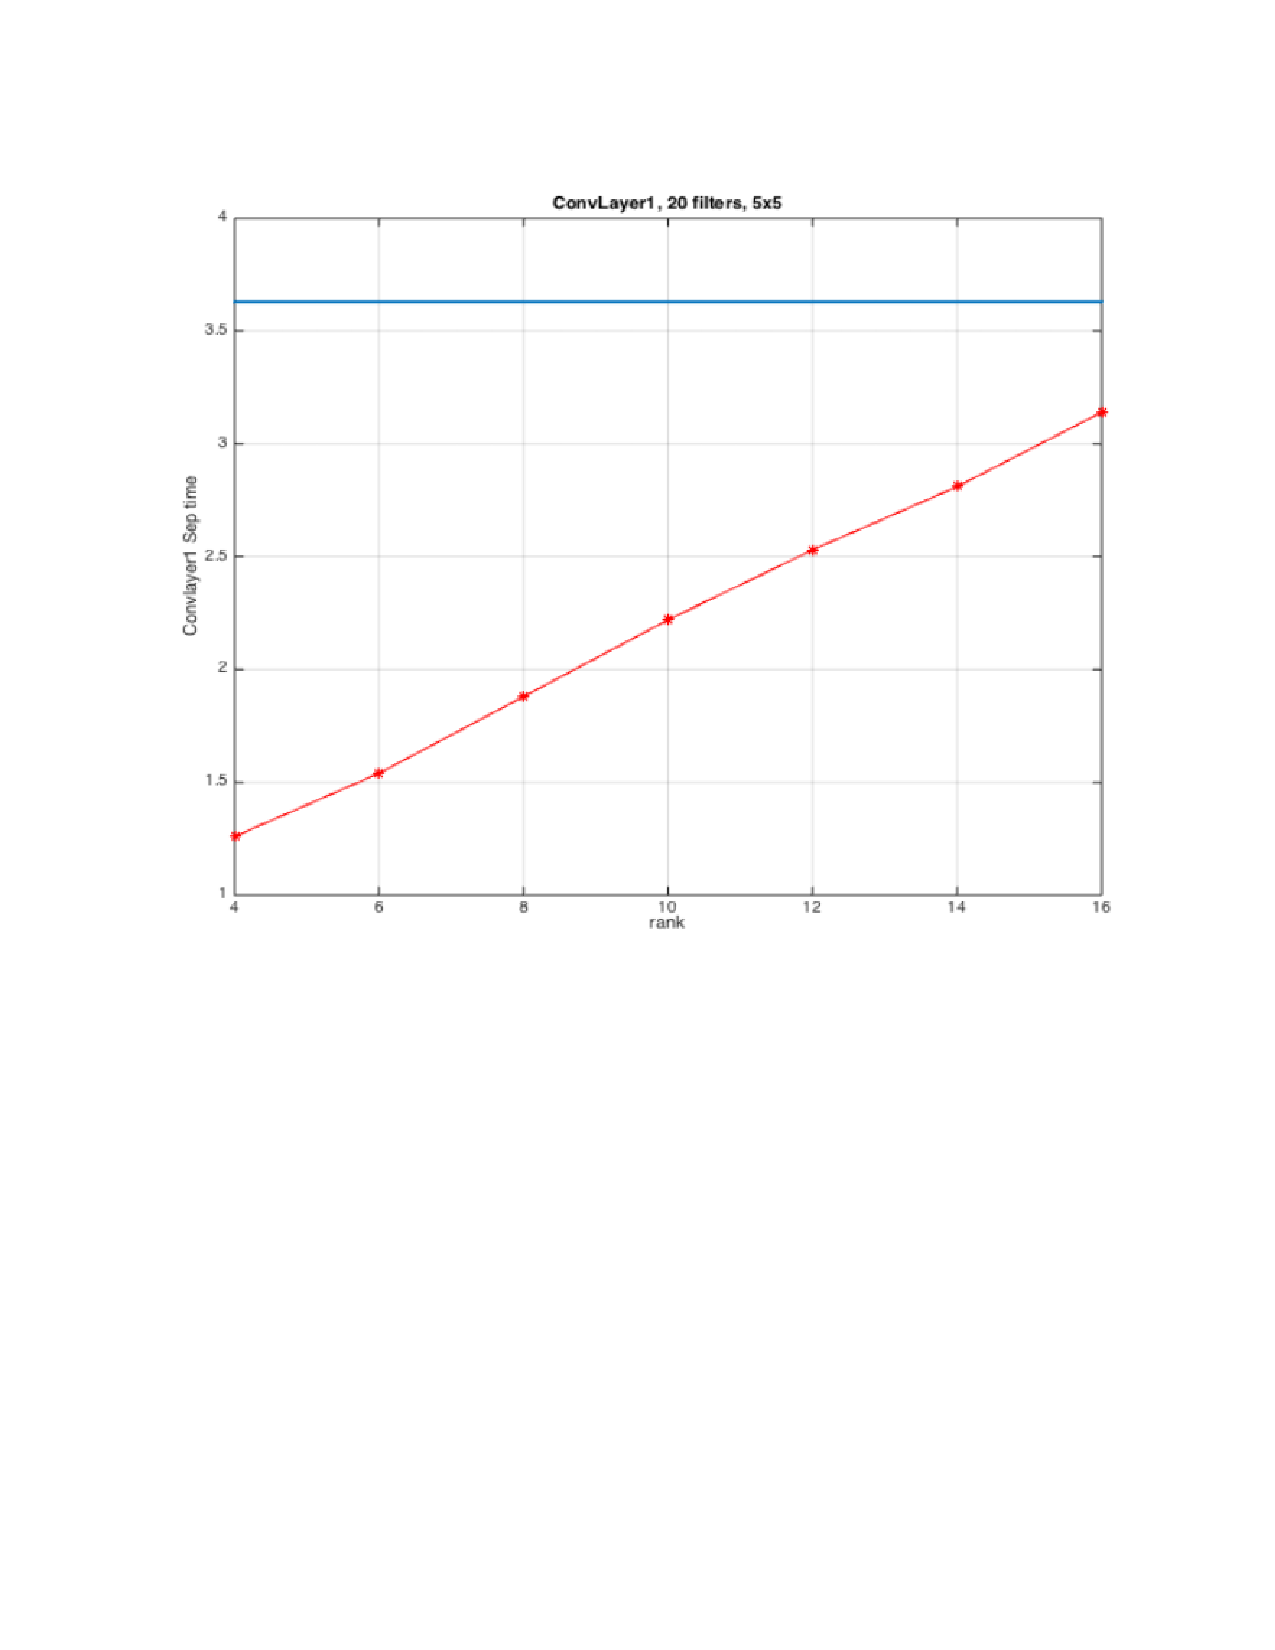
\includegraphics[width=\textwidth]{images/imagesCNN_page5.pdf}
    \caption{Convolutional layer 1}
  \end{subfigure}
  \begin{subfigure}[b]{0.40\textwidth}
    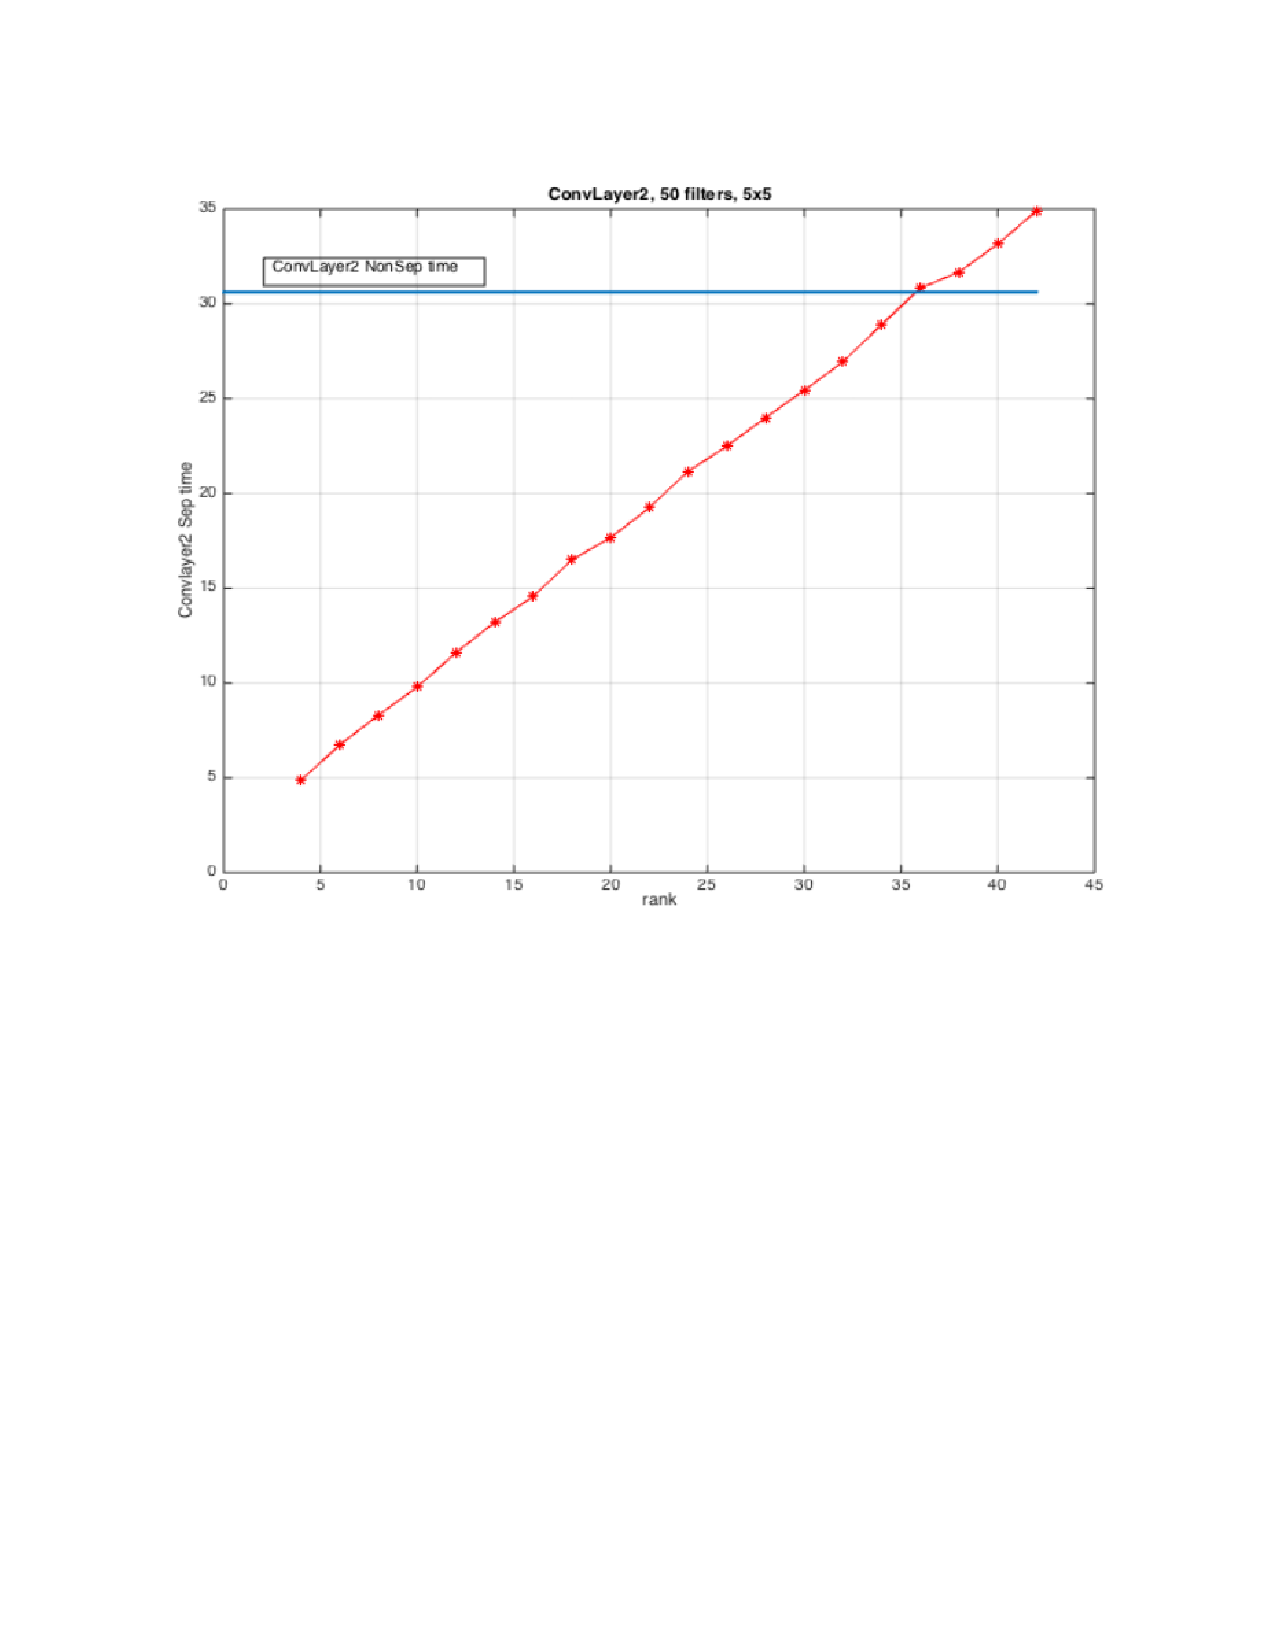
\includegraphics[width=\textwidth]{images/imagesCNN_page3.pdf}
    \caption{Convolutional layer 2}
  \end{subfigure}
  \caption{Rank vs Time}
  \label{fig:cnn1time}
\end{figure}

The question that remains now is to see how far can we afford to reduce the rank such that we do not lose much from the accuracy. Fig [cite]a shows how the performance of the CNN drops with decreasing rank. With rank 16 we do not
lose at all performance, while for rank between 10 and 16 the error rate stays between 0.8 and 0.9 per cent, which is quite low. According to the application, even a rank of 8 or 6 is acceptable, since the drop is not more than 1 per cent.

\begin{figure}[h]
  \centering
  \begin{subfigure}[b]{0.40\textwidth}
   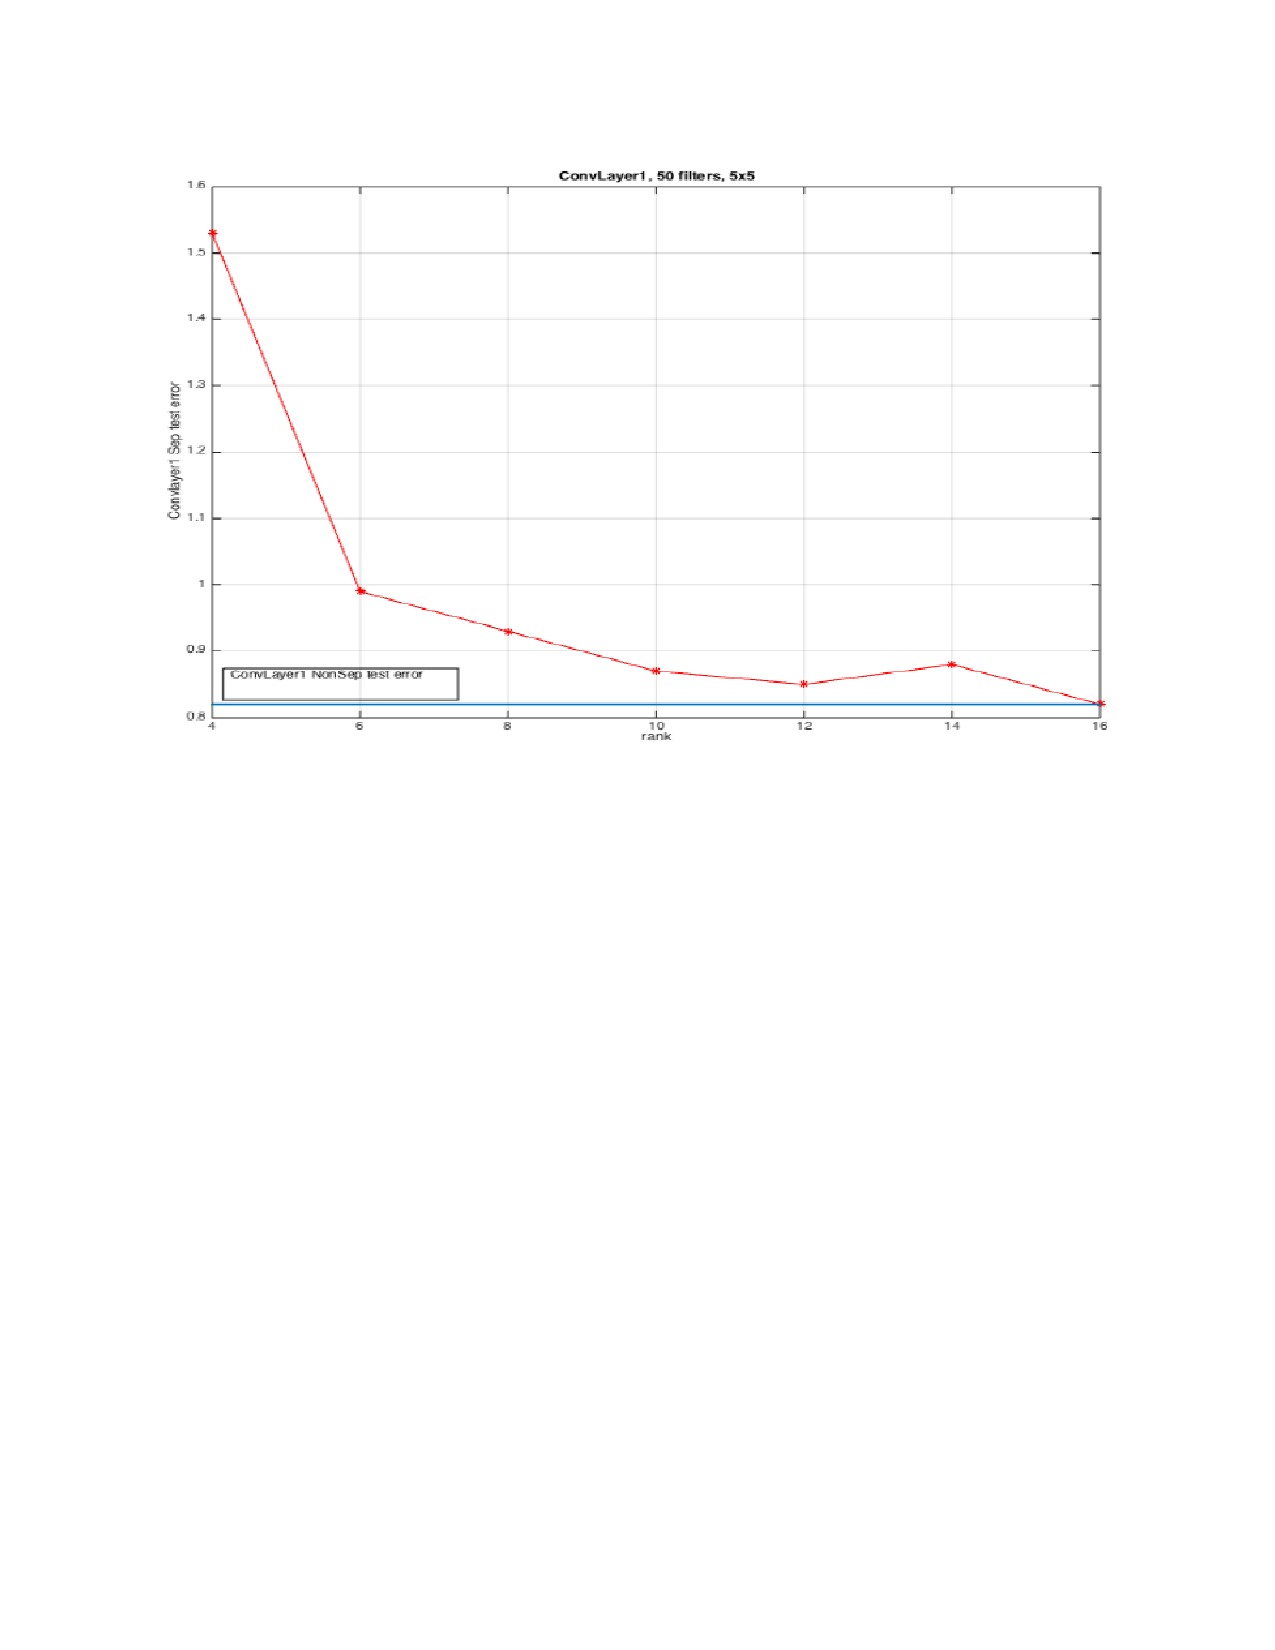
\includegraphics[width=\textwidth]{images/imagesCNN_page4.pdf}
    \caption{Convolutional layer 1}
  \end{subfigure}
  \begin{subfigure}[b]{0.40\textwidth}
    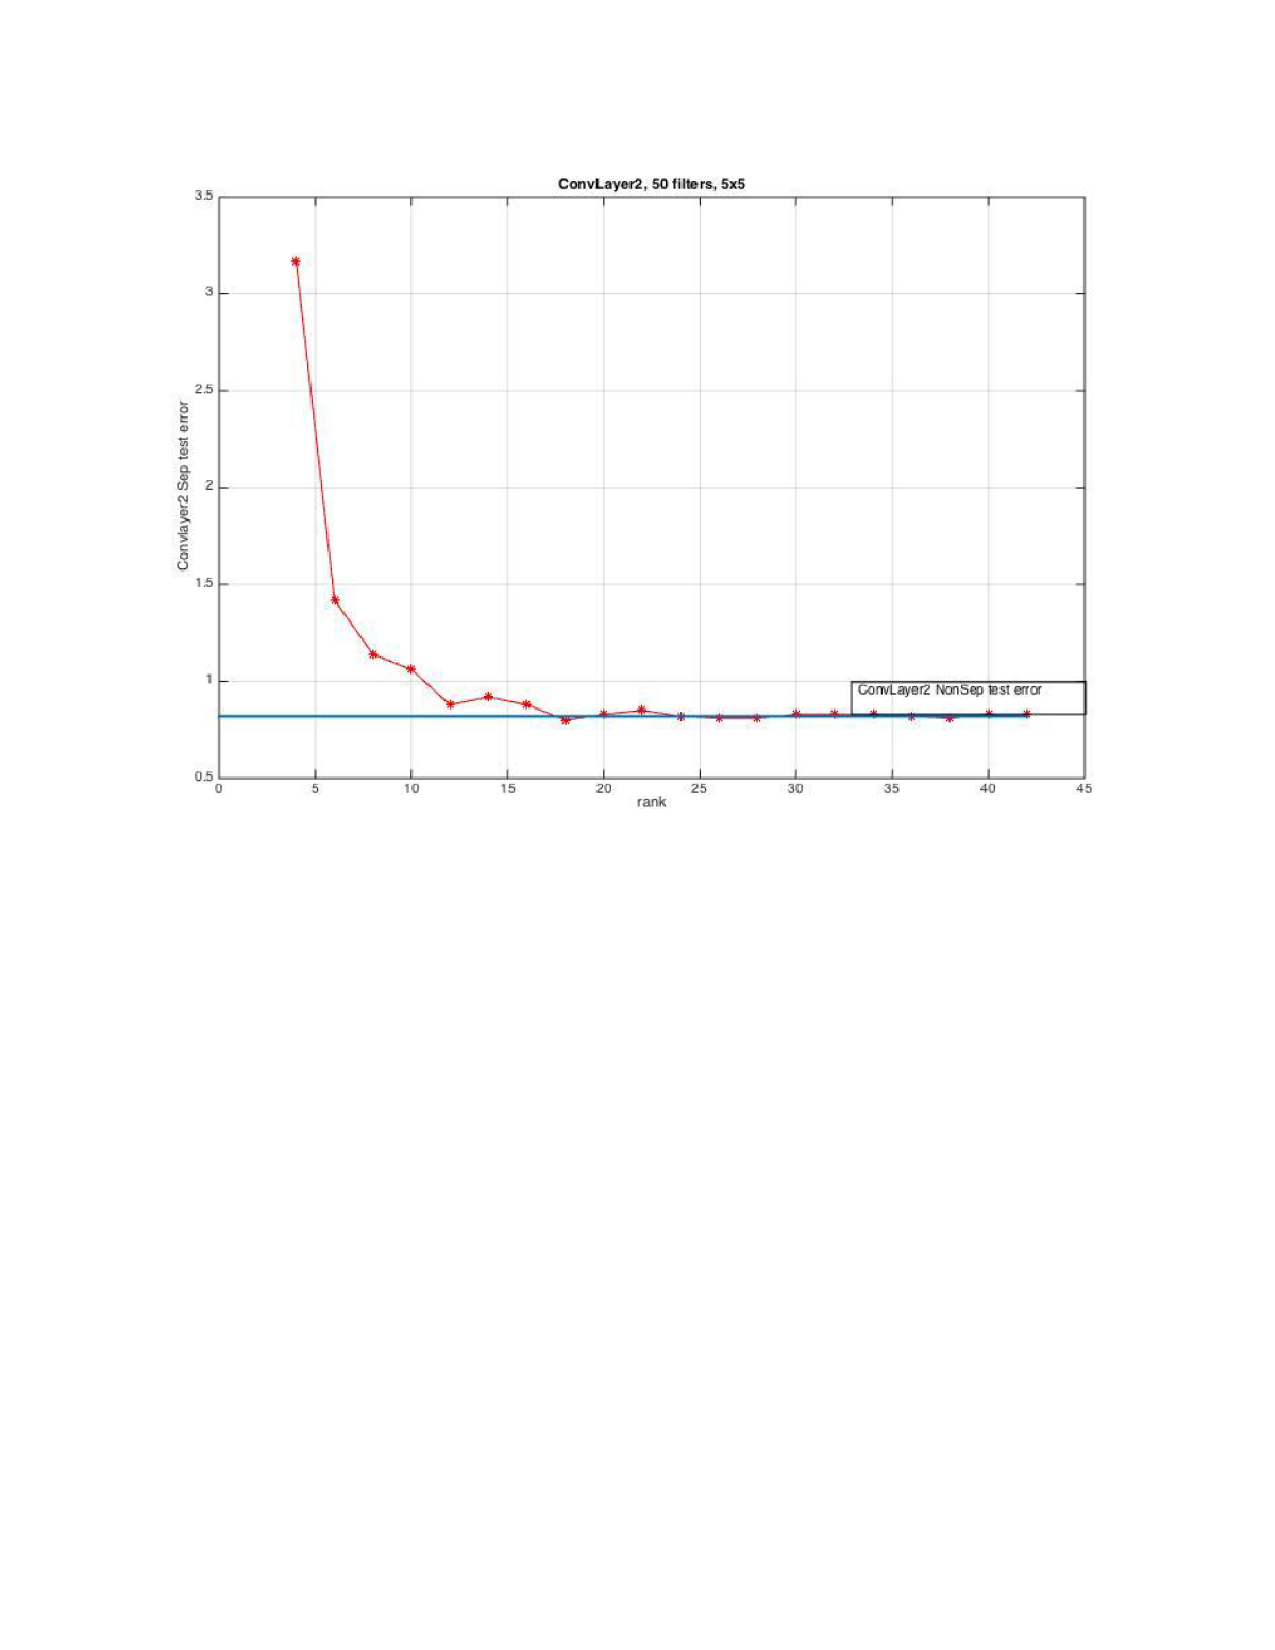
\includegraphics[width=\textwidth]{images/imagesCNN_page1.pdf}
    \caption{}
  \end{subfigure}
  \caption{Convolutional layer 2}
  \label{fig:cnn1error}
\end{figure}

We then kept the first layer fixed, and approximated the second layer.
Similarly as before, according to Table \ref{table:rank}, we have a very tall tensor $R^{50\times 5 \times 5}$ with a typical rank of 25.
Fig\ref{fig:cnn1fitness}b shows how well is the approximation with varying rank from 4 to 42 in steps of 2 . As expected, the fit is almost perfect (99.9 fit) for rank higher than the theoretical one of 25.

From the complexity perspective, the separable cnn is faster if we use a rank $K << \frac{Jd_{1}d_{2}}{J +d_{1}+d_{2}} = 20.83$. In our case, for rank = 20 we obtained almost a 40$\%$ speedup. This is due as before due to language specific implementation.
For rank 10, using separable filters is actually 3 times faster (theoretically 2 times faster).
If we keep the rank greater than 10, the recognition never drops more than 1 error rate.
For rank 12 the fit is 79 but the error rate is still almost unchanged which means we can easily use rank with not so perfect fit and still obtain good performance. The first layer with separable filters of similar fit of 79 obtain a slitghly lower performance.

\subsubsection{Model 2}

We use next a model with filters of size $9\times9$ for both layers.

\begin{table}
\centering
\begin{tabular}{@{}rlll@{}}\toprule
Layer & Type & Maps and neurons& Kernel size \\ \midrule
0 & input & 1 map of 28x28 &\\
1& convolutional & 20 maps of 24x24 & 9x9\\
2 & max pooling & 20 maps of 12x12 &  \\
3 & convolutional & 50 maps of 8x8& 9x9 \\
4 & max pooling & 50 maps of 4x4&  \\ 
5 & fully conntected& 500 & \\
6 & fully conntected & 2 neurons & \\ \bottomrule
\end{tabular}
\caption{Bigger CNN for MNIST set}
\label{fig:CNN2}
\end{table}

The theoretical rank is less than 49 and we obtain speedup if the rank $K << 59.5$
The results can be seen in the figure below

\begin{figure}[h]
  \centering
  \begin{subfigure}[b]{0.40\textwidth}
   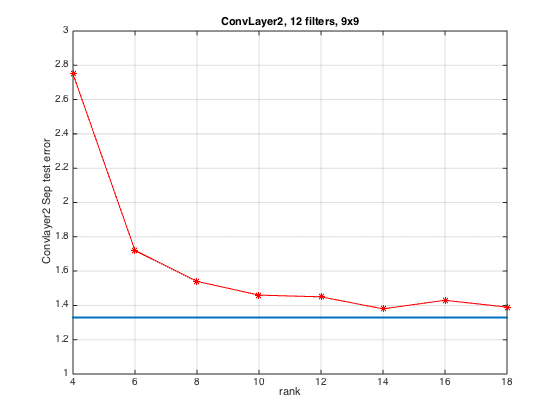
\includegraphics[width=\textwidth]{presentation_plots/convL2_error.png}
    \caption{Error vs Rank}
  \end{subfigure}
  \begin{subfigure}[b]{0.40\textwidth}
    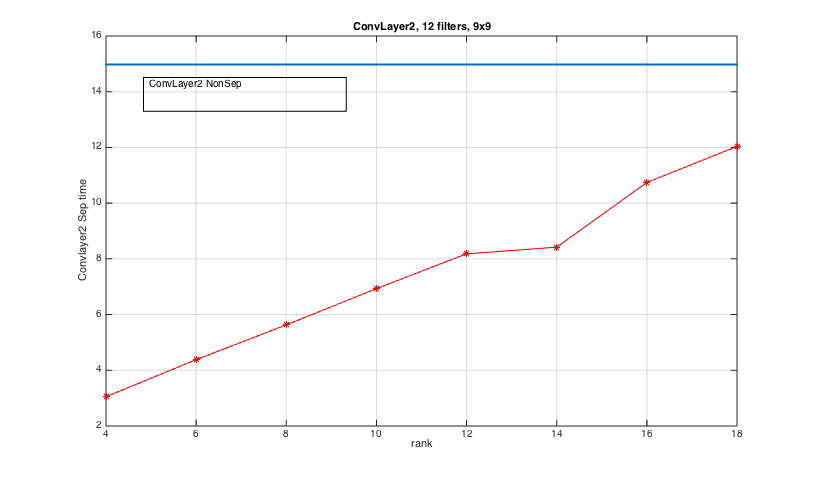
\includegraphics[width=\textwidth]{presentation_plots/convL2_time.png}
    \caption{Rank vs Time}
  \end{subfigure}
  \caption{Convolutional layer 2}
  \label{fig:cnn2error}
\end{figure}

\subsection{Mitocondria}

\begin{table}
\centering
\begin{tabular}{@{}rlll@{}}\toprule
Layer & Type & Maps and neurons& Kernel size \\ \midrule
0 & input & 1 map of 51x51 &\\
1& convolutional & 10 maps of 46x46 & 6x6\\
2 & max pooling & 10 maps of 23x23 &  \\
3 & convolutional & 20 maps of 18x18& 6x6 \\
4 & max pooling & 20 maps of 9x9& \\ 
3 & convolutional & 50 maps of 4x4& 6x6 \\
4 & max pooling & 50 maps of 2x2& \\ 
5 & fully conntected& 100 & \\
6 & fully conntected & 2 neurons & \\ \bottomrule
\end{tabular}
\caption{CNN for Mitocondria set}
\label{fig:CNN3}
\end{table}

\subsection{ImageNet}

\begin{figure}[h]
  \centering
  \begin{subfigure}[b]{0.40\textwidth}
   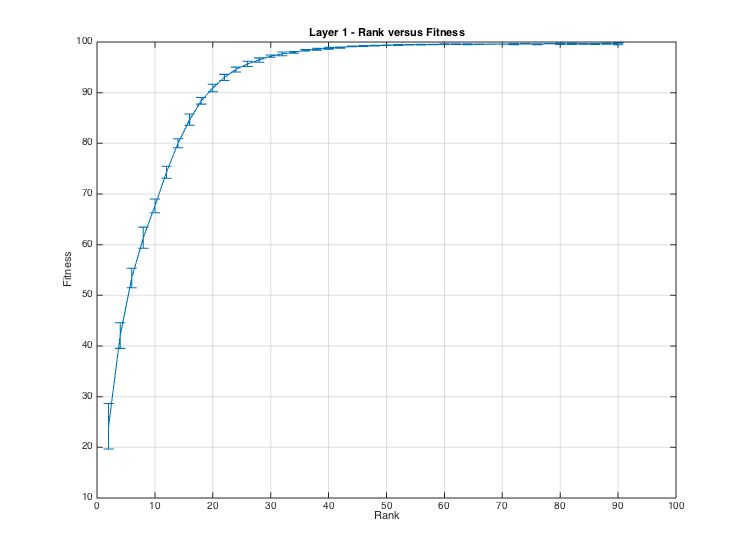
\includegraphics[width=\textwidth]{images/Layer1ImageNet.png}
    \caption{}
  \end{subfigure}
  \begin{subfigure}[b]{0.40\textwidth}
    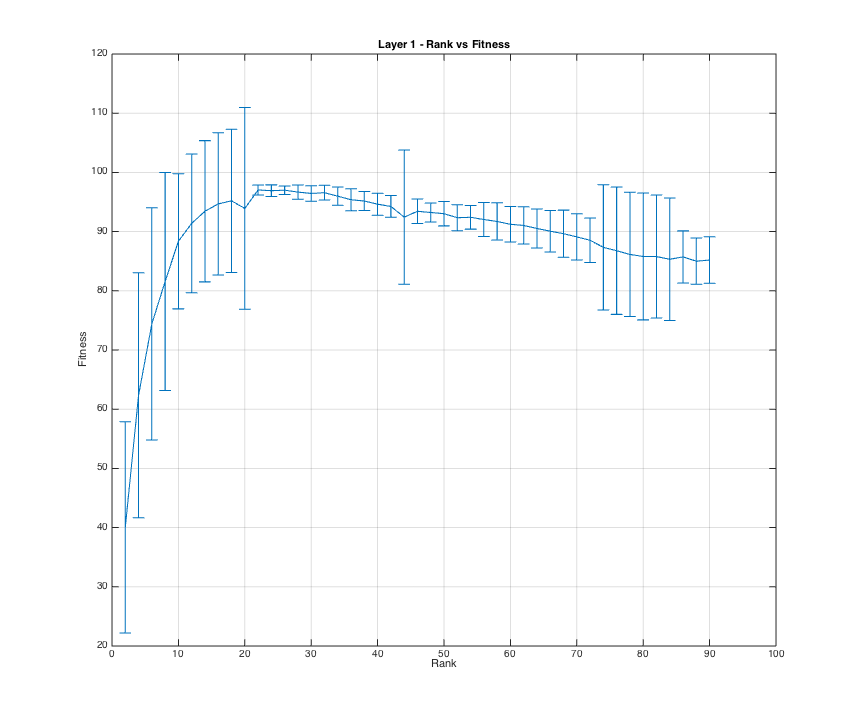
\includegraphics[width=\textwidth]{images/Layer2ImageNet.png}
    \caption{}
  \end{subfigure}
  \caption{ImageNet Layers}
  \label{fig:user_stribution}
\end{figure}

\begin{figure}[h]
  \centering
  \begin{subfigure}[b]{0.40\textwidth}
   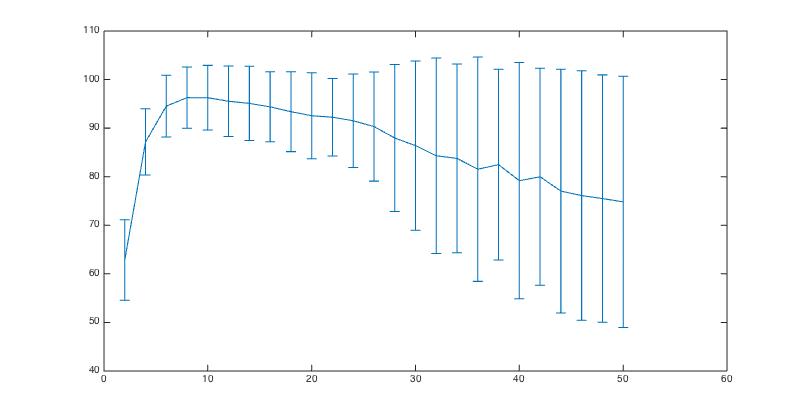
\includegraphics[width=\textwidth]{images/Layer3ImageNet.png}
    \caption{}
  \end{subfigure}
  \begin{subfigure}[b]{0.40\textwidth}
    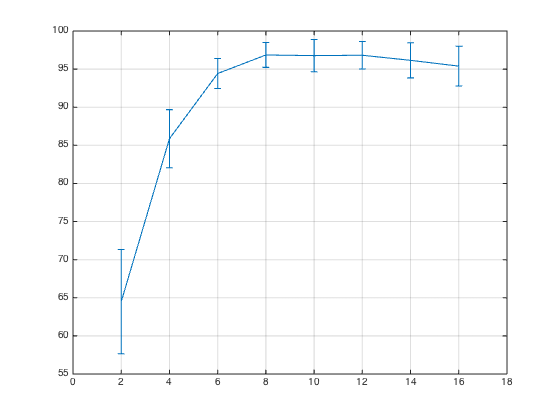
\includegraphics[width=\textwidth]{images/Layer4ImageNet.png}
    \caption{}
  \end{subfigure}
  \caption{ImageNet Layers}
  \label{fig:user_artiststribution}
\end{figure}

\section{Conclusions}
Theoretical bounds of the separabe filters choice are proven.
Impreved recognition on mitocondria set.

\section*{Acknowledgments}
We would like to thank Simon Arosi that helped me a lot during this project giving me constant feedback.

\bibliography{citations}
\bibliographystyle{plain}

\end{document}

